\chapter{Wellenfunktionen, Dichtematrizen und Lokalität}

\lectureoverview{Der Satz von Bell wird aus einem wesentlichen Grund zurückgestellt: Bevor wir fragen, was Bell verbietet, müssen wir genau sagen, was Verschränkung ist. Ein bipartiter Zustand ist verschränkt, wenn er sich nicht in einen Zustand für Alice und einen für Bob faktorisieren lässt. Wellenfunktionen machen dieses Kriterium konkret, Korrelationen zeigen seine Folgen, und der Singulettzustand liefert das entscheidende Beispiel. Die reduzierte Dichtematrix wird dann zur vollständigen lokalen Beschreibung eines Teils eines verschränkten Ganzen. Mit diesem Instrumentarium erscheint die Messung als verschränkende Wechselwirkung; die System--Beobachter-Grenze lässt sich verschieben, ohne die Vorhersagen zu ändern, und die scheinbare Spannung zwischen Verschränkung und Lokalität lässt sich präzise formulieren: Entfernte Entscheidungen verändern bedingte Korrelationen, nicht aber die unbedingten Statistiken, die zur Signalübertragung verfügbar sind.}

\section{Was Verschränkung tatsächlich bedeutet}

Es liegt nahe, direkt zum Satz von Bell überzugehen. Der Satz ist elegant, doch seine Bedeutung lässt sich nicht von der Struktur trennen, die er prüft. Die dringendere Frage lautet daher noch nicht, ob die Quantenmechanik eine Bell-Ungleichung verletzt, sondern was ein verschränkter Zustand über ein zusammengesetztes System aussagt.

Eine gängige Formulierung besagt, dass zwei verschränkte Systeme \emph{einen Zustand teilen}. Diese Formulierung unterscheidet jedoch nichts. Jedes zusammengesetzte System hat einen Zustand, ob verschränkt oder nicht. Entscheidend ist die Faktorisierbarkeit. Haben \(A\) und \(B\) die Hilberträume \(\mathcal H_A\) und \(\mathcal H_B\), so liegt der Zustand des Paars in
\begin{equation}
\mathcal H_{AB}=\mathcal H_A\otimes\mathcal H_B.
\end{equation}
Ein reiner Zustand ist ein Produktzustand, wenn er sich schreiben lässt als
\begin{equation}
\ket{\Psi}_{AB}=\ket{\psi}_A\otimes\ket{\phi}_B.
\label{eq:l7-product-state}
\end{equation}
Existiert kein solches Faktorenpaar, ist \(\ket{\Psi}_{AB}\) verschränkt.

\begin{classroomqa}
\audiencequestion{Bedeutet Verschränkung einfach, dass beide Systeme in einem Zustandsvektor vorkommen?}
\lecturerresponse{Nein. Auch ein Produktzustand gehört zum Hilbertraum des gesamten Paars. Verschränkung ist die stärkere, basisunabhängige Aussage, dass sich der Vektor des Ganzen nicht als Vektor für Alice mal Vektor für Bob schreiben lässt.}
\end{classroomqa}

\begin{classroomqa}
\audiencequestion{Kann eine geschickte Basisänderung einen verschränkten Zustand in einen Produktzustand verwandeln?}
\lecturerresponse{Nicht, wenn die Basisänderung lokal ist, also aus einer Basisänderung für Alice und einer weiteren für Bob besteht. Lokale Basisänderungen verändern die Koordinaten der einzelnen Faktoren, nicht aber die Frage, ob der Zustand faktorisiert. Eine völlig beliebige Basis des gemeinsamen Hilbertraums kann die Tensorproduktstruktur verschleiern, ändert aber nicht, welche physikalischen Freiheitsgrade zu Alice und Bob gehören.}
\end{classroomqa}

\section{Wellenfunktionen als Koordinaten im Hilbertraum}

Der Begriff \emph{Wellenfunktion} weckt historische Vorstellungen, die nicht zu seiner mathematischen Definition gehören. Eine Wellenfunktion ist die Koordinatendarstellung eines Zustandsvektors in einer gewählten Basis. Eine vollständige Menge kommutierender Observablen habe die gemeinsamen Eigenvektoren
\begin{equation}
\ket{a,b,c,\ldots}.
\end{equation}
Die Bezeichnungen müssen vollständig sein: Zusammengenommen unterscheiden sie jeden Vektor der Basis. Dann gilt
\begin{align}
\ket{\Psi}
&=\sum_{a,b,c,\ldots}
\ket{a,b,c,\ldots}
\braket{a,b,c,\ldots}{\Psi} \\
&=\sum_{a,b,c,\ldots}
\psi(a,b,c,\ldots)\ket{a,b,c,\ldots},
\label{eq:l7-wavefunction-expansion}
\end{align}
mit
\begin{equation}
\psi(a,b,c,\ldots)
=\braket{a,b,c,\ldots}{\Psi}.
\label{eq:l7-wavefunction-definition}
\end{equation}
Bei kontinuierlichen Bezeichnungen werden die entsprechenden Summen zu Integralen.

\begin{figure}[htbp]
\centering
\includegraphics[width=0.88\textwidth]{lecture_07_figure_01.png}
\caption{Die Wellenfunktion als Menge der Koeffizienten eines Zustands bezüglich einer vollständigen Basis.}
\lectureframe{00:07:00}
\end{figure}

Für ein Teilchen im dreidimensionalen Raum können \(x,y,z\) die kommutierenden Bezeichnungen sein, und
\begin{equation}
\psi(x,y,z)=\braket{x,y,z}{\Psi}
\end{equation}
ist die vertraute Ortsraum-Wellenfunktion von Schr\"odinger. Für einen Spin in der Basis \(\sigma_z\) besteht die Wellenfunktion lediglich aus dem Paar
\begin{equation}
\psi(u)=\braket{u}{\Psi},
\qquad
\psi(d)=\braket{d}{\Psi}.
\end{equation}
Für zwei Spins benötigt man zwei Bezeichnungen:
\begin{equation}
\Psi(a,b)=\braket{a,b}{\Psi},
\qquad
a,b\in\{u,d\}.
\label{eq:l7-two-spin-wavefunction}
\end{equation}
Diese Definition setzt keine buchstäbliche Welle im Raum voraus.

\begin{classroomqa}
\audiencequestion{Ist ein Wechsel der Wellenfunktionsbasis eine Fourier-Transformation?}
\lecturerresponse{Eine Fourier-Transformation ist die spezielle Basisänderung zwischen Orts- und Impulsdarstellung. Allgemeiner ist jeder Wechsel zwischen orthonormalen Basen eine unitäre Transformation der Koordinaten. Der Übergang von der Basis \(\sigma_z\) zur Basis \(\sigma_x\) ist mit einer Fourier-Transformation vergleichbar, auch wenn es sich dabei um eine endlichdimensionale unitäre Matrix und nicht um die Orts--Impuls-Integraltransformation handelt.}
\end{classroomqa}

\begin{classroomqa}
\audiencequestion{Hat sich der physikalische Zustand geändert, wenn sich die Wellenfunktion bei einer Basisänderung ändert?}
\lecturerresponse{Nein. Das Ket \(\ket{\Psi}\) ist der abstrakte Zustand. Die Zahlen \(\psi(a,b,c,\ldots)\) sind seine Koordinaten in einer ausgewählten Basis. Bei einem Koordinatenwechsel ändern sich diese Zahlen, während der Vektor und alle physikalischen Vorhersagen gleich bleiben.}
\end{classroomqa}

\section{Erwartungswerte in Komponenten}

Bevor wir Dichtematrizen einführen, betrachten wir die Komponentenstruktur eines Erwartungswerts. Sei \(L\) eine Observable mit Matrixelementen
\begin{equation}
L_{a'a}=\bra{a'}L\ket{a}.
\label{eq:l7-matrix-elements}
\end{equation}
Für \(\ket{\Psi}=\sum_a\psi(a)\ket{a}\) gilt dann
\begin{align}
\expect{L}
&=\bra{\Psi}L\ket{\Psi} \\
&=\sum_{a',a}
\psi^*(a')\bra{a'}L\ket{a}\psi(a) \\
&=\sum_{a',a}\psi^*(a')L_{a'a}\psi(a).
\label{eq:l7-expectation-components}
\end{align}

\begin{figure}[htbp]
\centering
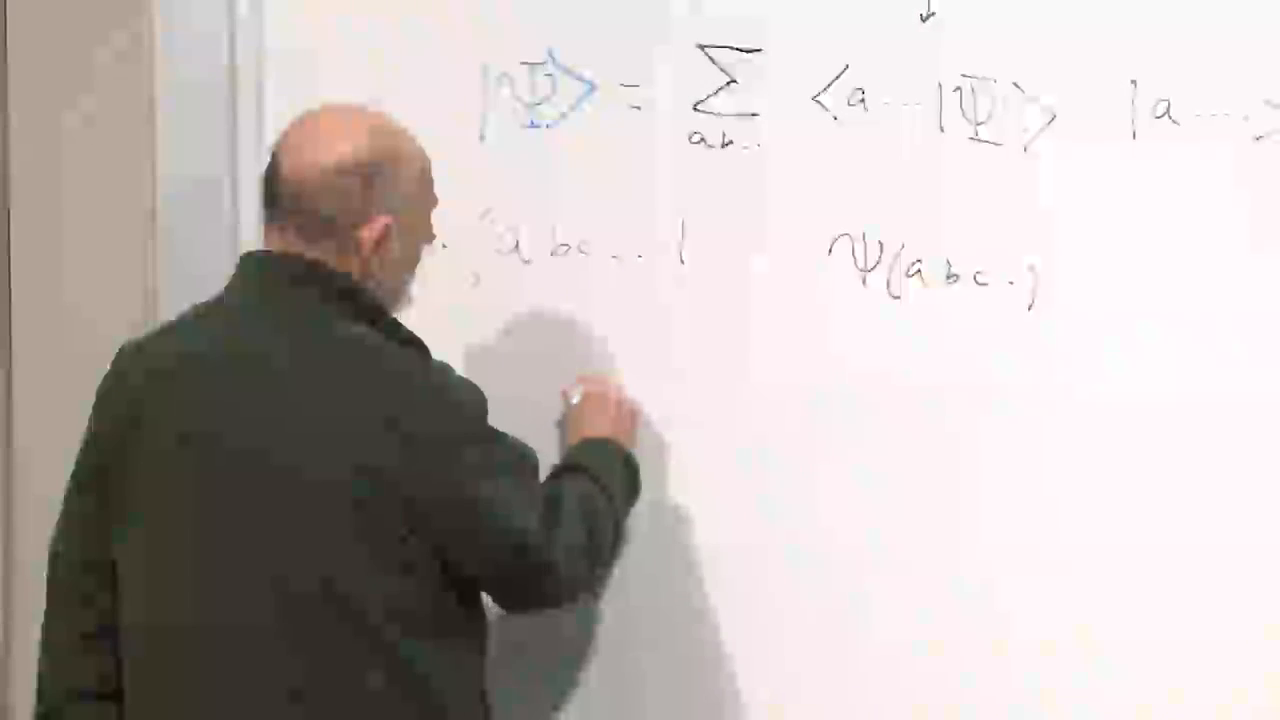
\includegraphics[width=0.88\textwidth]{lecture_07_figure_02.png}
\caption{Der Erwartungswert-Sandwich, ausgedrückt durch Wellenfunktionskoeffizienten und Matrixelemente.}
\lectureframe{00:14:08}
\end{figure}

Nun teilen wir das System in Alice' Teil und Bobs Teil auf. Sei \(a\) eine vollständige Basisbezeichnung für Alice und \(b\) eine für Bob:
\begin{equation}
\ket{\Psi}_{AB}
=\sum_{a,b}\Psi(a,b)\ket{a,b}.
\label{eq:l7-composite-expansion}
\end{equation}
Eine Observable, die ausschließlich zu Alice gehört, wird im zusammengesetzten Raum dargestellt durch
\begin{equation}
L_A=L\otimes I_B,
\end{equation}
Ihre Matrixelemente lauten daher
\begin{equation}
\bra{a',b'}L_A\ket{a,b}
=L_{a'a}\delta_{b'b}.
\label{eq:l7-alice-local-matrix}
\end{equation}
Entsprechend hat eine lokale Observable von Bob die Form
\begin{equation}
M_B=I_A\otimes M,
\qquad
\bra{a',b'}M_B\ket{a,b}
=\delta_{a'a}M_{b'b}.
\label{eq:l7-bob-local-matrix}
\end{equation}
Die Identität im unberührten Faktor bringt mathematisch zum Ausdruck, dass Alice' Operation auf Alice und Bobs Operation auf Bob wirkt.

Setzt man Gleichung~\eqref{eq:l7-alice-local-matrix} in den Erwartungswert ein, erhält man
\begin{equation}
\expect{L_A}
=\sum_{a',a,b}
\Psi^*(a',b)L_{a'a}\Psi(a,b).
\label{eq:l7-local-expectation}
\end{equation}
Diese Formel enthält bereits die reduzierte Dichtematrix; wir ordnen sie später um, nachdem wir zunächst betrachtet haben, was die Faktorisierung bewirkt.

\begin{classroomqa}
\audiencequestion{Warum bleibt in Gleichung~\eqref{eq:l7-local-expectation} nur ein Bob-Index übrig?}
\lecturerresponse{Die Identität im Hilbertraum von Bob liefert \(\delta_{b'b}\). Dadurch werden die Bra- und Ket-Bezeichnungen auf Bobs Seite gleichgesetzt, sodass die Doppelsumme über \(b',b\) zu einer Summe über \(b\) wird.}
\end{classroomqa}

\begin{classroomqa}
\audiencequestion{Muss Alice wissen, welche Basis Bob verwendet?}
\lecturerresponse{Keine physikalische Vorhersage hängt von Bobs Basis ab. Die Summe über eine vollständige Bob-Basis ist eine Auflösung der Identität. Eine andere Basis von Bob ändert die einzelnen Komponenten \(\Psi(a,b)\), nicht aber Alice' Erwartungswert.}
\end{classroomqa}

\section{Produktzustände und Korrelationen}

In einem Produktzustand faktorisiert die gemeinsame Wellenfunktion:
\begin{equation}
\Psi(a,b)=\psi_A(a)\phi_B(b).
\label{eq:l7-wavefunction-factorization}
\end{equation}
Setzt man dies in Gleichung~\eqref{eq:l7-local-expectation} ein, erhält man:
\begin{align}
\expect{L_A}
&=\sum_{a',a,b}
\psi_A^*(a')\phi_B^*(b)
L_{a'a}
\psi_A(a)\phi_B(b) \\
&=\left[
\sum_{a',a}\psi_A^*(a')L_{a'a}\psi_A(a)
\right]
\left[
\sum_b|\phi_B(b)|^2
\right] \\
&=\bra{\psi_A}L\ket{\psi_A}.
\label{eq:l7-product-local-expectation}
\end{align}
Aufgrund der Normierung von Bob ist sein Faktor gleich eins. Alice hat daher genau dieselben lokalen Statistiken wie ohne Bobs System.

\begin{figure}[htbp]
\centering
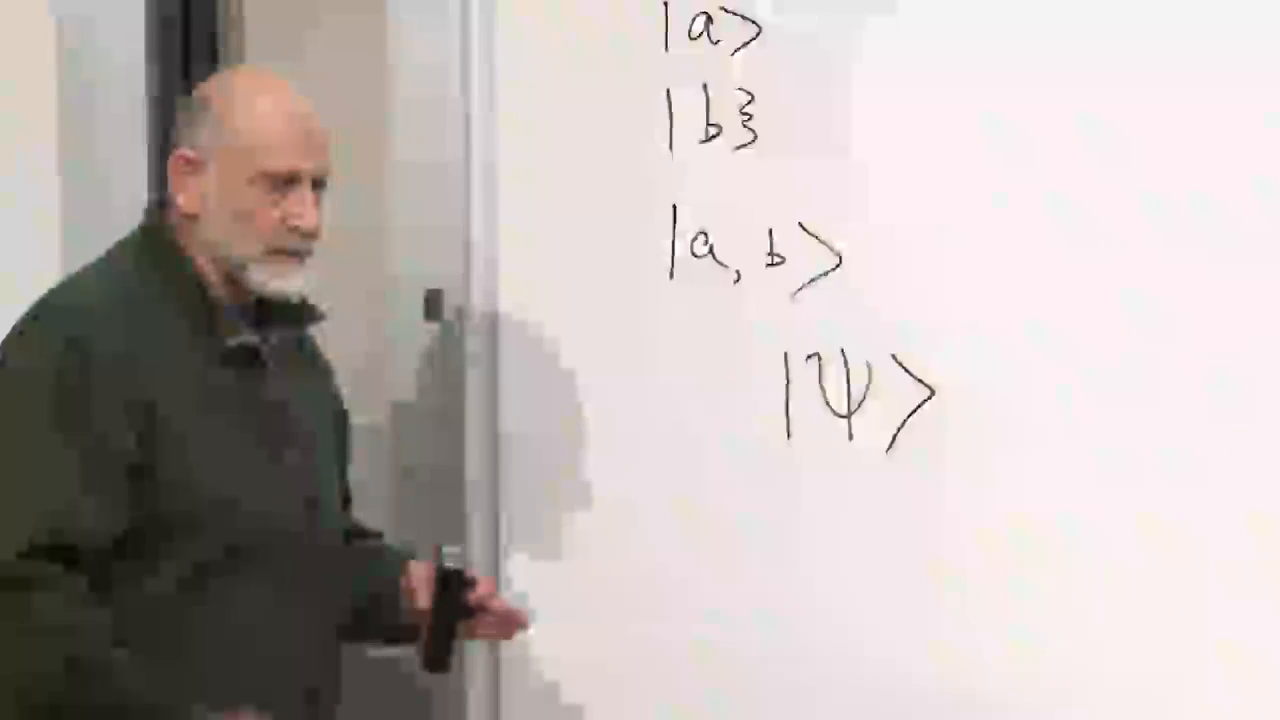
\includegraphics[width=0.88\textwidth]{lecture_07_figure_03.png}
\caption{Faktorisierung der gemeinsamen Wellenfunktion und die entsprechende Zerlegung lokaler Erwartungswerte.}
\lectureframe{00:29:18}
\end{figure}

Das Produkt einer Alice-Observable und einer Bob-Observable hat die Matrixelemente
\begin{equation}
\bra{a',b'}L_A M_B\ket{a,b}
=L_{a'a}M_{b'b}.
\end{equation}
In einem Produktzustand zerfällt sein Erwartungswert:
\begin{equation}
\expect{L_A M_B}
=\expect{L_A}\expect{M_B}.
\label{eq:l7-product-correlation-factorization}
\end{equation}
Daher ist es naheliegend, die verbundene Korrelation zu definieren als
\begin{equation}
C(L,M)
=\expect{L_A M_B}
-\expect{L_A}\expect{M_B}.
\label{eq:l7-connected-correlation}
\end{equation}
Für jeden Produktzustand gilt \(C(L,M)=0\) für jedes Paar lokaler Observablen. Umgekehrt garantiert die Verschränkung eines reinen bipartiten Zustands, dass es ein Paar lokaler Observablen mit einer von null verschiedenen verbundenen Korrelation gibt.

\begin{classroomqa}
\audiencequestion{Bedeutet \(L_A M_B\), dass Bob zuerst und Alice danach gemessen wird?}
\lecturerresponse{Nein. Operatoren wirken auf Zustandsvektoren; Messungen werden von Messapparaturen durchgeführt. Das Produkt bedeutet, dass zuerst \(M_B\) und danach \(L_A\) wirkt. Da die Operatoren zu verschiedenen Tensorfaktoren gehören, gilt \([L_A,M_B]=0\); ihre mathematische Reihenfolge ist daher unerheblich. Ein Laborverfahren zur Bestimmung des gemeinsamen Erwartungswerts ist eine davon getrennte Frage.}
\end{classroomqa}

\begin{classroomqa}
\audiencequestion{Kann der Zustand verschränkt sein, obwohl eine ausgewählte Korrelation verschwindet?}
\lecturerresponse{Gewiss. Ein verschwindendes \(C(L,M)\) besagt lediglich, dass dieses bestimmte Observablepaar unkorreliert ist. Um die Faktorisierbarkeit eines reinen Zustands festzustellen, müssen sich alle lokalen Kreuzkorrelationen faktorisieren lassen. Eine teilweise Korrelation muss auch nicht bedeuten, dass eine einfache einzelne Zahl den Grad der Verschränkung angibt; darüber gibt das gesamte Spektrum der reduzierten Dichtematrix Auskunft.}
\end{classroomqa}

\begin{classroomqa}
\audiencequestion{Ist jeder korrelierte Zustand verschränkt?}
\lecturerresponse{Bei den hier betrachteten reinen Zuständen weisen nichtfaktorisierende Korrelationen auf Verschränkung hin. Bei gemischten Zuständen können gewöhnliche klassische Korrelationen ebenfalls dazu führen, dass \(C(L,M)\neq0\). Das spätere Dichtematrix-Kriterium muss daher danach qualifiziert werden, ob der Zustand des Ganzen bekanntermaßen rein ist.}
\end{classroomqa}

\section{Der Singulettzustand: ein bestimmtes Ganzes mit unbestimmten Teilen}

Sei \(\boldsymbol{\sigma}\) der Operator für Bobs Spin und \(\boldsymbol{\tau}\) der für Alice'. Ihr Singulettzustand lautet
\begin{equation}
\ket{S}
=\frac{1}{\sqrt2}
\left(\ket{u d}-\ket{d u}\right),
\label{eq:l7-singlet}
\end{equation}
wobei der erste Platz Bob und der zweite Alice zugeordnet ist. Keiner der beiden Spins hat eine bestimmte \(z\)-Komponente:
\begin{equation}
\expect{\sigma_z}=0,
\qquad
\expect{\tau_z}=0.
\label{eq:l7-singlet-local-z}
\end{equation}
Ihr Produkt ist dagegen sicher:
\begin{equation}
\expect{\sigma_z\tau_z}=-1.
\label{eq:l7-singlet-product-z}
\end{equation}
Jede \(z\)-Messung ergibt entgegengesetzte Resultate.

Wegen der Rotationsinvarianz hängt diese Aussage nicht von der Richtung ab. Für jeden Einheitsvektor \(\mathbf n\) gilt
\begin{equation}
\expect{\boldsymbol{\sigma}\cdot\mathbf n}
=\expect{\boldsymbol{\tau}\cdot\mathbf n}=0,
\qquad
\expect{
(\boldsymbol{\sigma}\cdot\mathbf n)
(\boldsymbol{\tau}\cdot\mathbf n)
}=-1.
\label{eq:l7-singlet-any-axis}
\end{equation}
Allgemeiner gilt
\begin{equation}
\expect{\sigma_i\tau_j}=-\delta_{ij}.
\label{eq:l7-singlet-correlation-tensor}
\end{equation}
Jeder Teil ist vollständig unpolarisiert, während die Resultate entlang gleicher Achsen perfekt antikorreliert sind.

\begin{figure}[htbp]
\centering
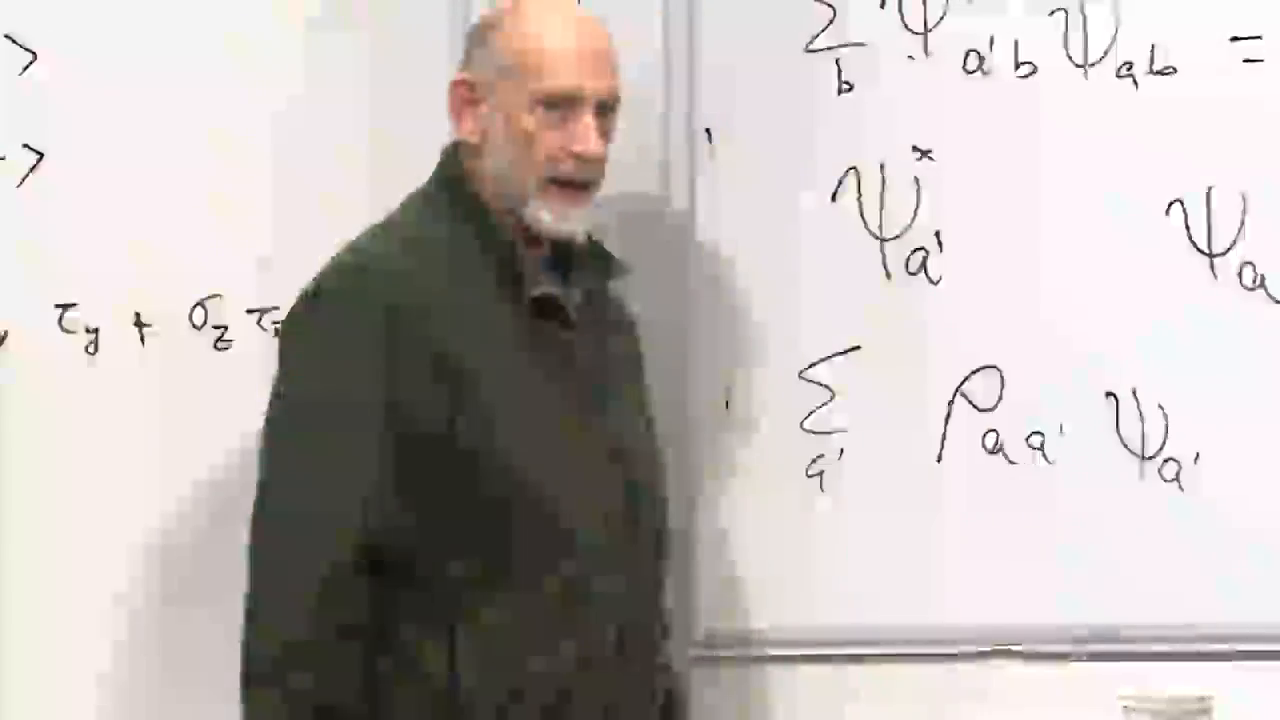
\includegraphics[width=0.88\textwidth]{lecture_07_figure_04.png}
\caption{Im Singulettzustand verschwindet jeder lokale Spinmittelwert, während gleiche Komponenten das Produkt \(-1\) haben.}
\lectureframe{00:38:28}
\end{figure}

Dies ist die charakteristische Umkehrung, die durch Verschränkung entsteht. Für einen isolierten Spin in einem reinen Zustand gibt es eine Richtung, entlang derer sein Spin bestimmt ist. Im Singulettzustand gibt es keine Richtung, entlang derer einer der lokalen Spins bestimmt wäre. Dennoch ist der zusammengesetzte Zustand rein und vollständig festgelegt. Wir wissen über das Ganze so viel, wie die Quantenmechanik erlaubt, und können trotzdem keinem der beiden Teile einen reinen Zustand zuweisen.

\begin{classroomqa}
\audiencequestion{Wenn der Zustand des Ganzen genau bekannt ist, warum können wir dann nicht für jeden Spin einen bestimmten Zustand ableiten?}
\lecturerresponse{Weil der Singulettzustand kein Produktzustand ist. Seine Koeffizienten lassen sich nicht in eine Bob-Amplitude mal eine Alice-Amplitude zerlegen. Die Information steckt in den Beziehungen zwischen den Teilen und nicht in zwei unabhängig existierenden lokalen Wellenfunktionen.}
\end{classroomqa}

\begin{classroomqa}
\audiencequestion{Kann ein Operator wie \(\sigma_z\) selbst ein möglicher Zustand des Spins sein?}
\lecturerresponse{Nein. Ein Zustand ist ein Vektor oder allgemeiner ein Dichteoperator; \(\sigma_z\) ist eine Observable, die auf Zustände wirkt. Ein Eigenvektor von \(\sigma_z\) ist ein Zustand mit einer bestimmten \(z\)-Komponente, aber die Observable und ihre Eigenvektoren sind unterschiedliche Arten von Objekten.}
\end{classroomqa}

\begin{classroomqa}
\audiencequestion{Haben wir eine Messung vorgenommen, wenn wir \(\sigma_z\tau_z\ket{S}=-\ket{S}\) schreiben?}
\lecturerresponse{Nein. Die Gleichung hält fest, wie ein Operator auf einen Vektor wirkt. Sie besagt, dass eine Messung der entsprechenden gemeinsamen Observablen mit Sicherheit \(-1\) ergeben würde; allein durch das Aufschreiben der Eigenwertgleichung wurde jedoch kein Detektor einbezogen.}
\end{classroomqa}

\begin{classroomqa}
\audiencequestion{Kann ein verschränktes Paar nur teilweise korreliert sein?}
\lecturerresponse{Ja. Perfekte Antikorrelation ist eine besondere Eigenschaft des Singulettzustands bei gleichen Achsen. Andere verschränkte Zustände können schwächere Korrelationen aufweisen, und auch beim Singulettzustand erhält man bei unterschiedlichen Achsen \(-\mathbf a\cdot\mathbf b\) statt \(-1\). Verschränkung betrifft die Nichtfaktorisierbarkeit, nicht perfekte Übereinstimmung oder Nichtübereinstimmung bei jeder ausgewählten Messung.}
\end{classroomqa}

\section{Präparation des Singulettzustands durch Energieabgabe}

Der rotationsinvariante Operator für zwei Spins
\begin{equation}
\boldsymbol{\sigma}\cdot\boldsymbol{\tau}
=\sigma_x\tau_x+\sigma_y\tau_y+\sigma_z\tau_z
\label{eq:l7-spin-dot-spin}
\end{equation}ordnet den vierdimensionalen Zustandsraum. Für den Singulettzustand gilt
\begin{equation}
(\boldsymbol{\sigma}\cdot\boldsymbol{\tau})\ket{S}
=-3\ket{S},
\label{eq:l7-singlet-dot-eigenvalue}
\end{equation}
während jeder der drei Triplettzustände den Eigenwert \(+1\) hat.

\begin{figure}[htbp]
\centering
\includegraphics[width=0.88\textwidth]{lecture_07_figure_05.png}
\caption{Die rotationsinvariante Kopplung \(\boldsymbol{\sigma}\cdot\boldsymbol{\tau}\) und ihre Rolle bei der Trennung von Singulett- und Triplettsektoren.}
\lectureframe{00:52:33}
\end{figure}

Angenommen, der Wechselwirkungs-Hamiltonoperator enthält
\begin{equation}
H_{\mathrm{int}}
=J\,\boldsymbol{\sigma}\cdot\boldsymbol{\tau}.
\label{eq:l7-exchange-hamiltonian}
\end{equation}
Bei antiferromagnetischer Kopplung \(J>0\) liegt der Singulettzustand um
\begin{equation}
\Delta E=4J.
\end{equation}unterhalb des Tripletts. Bringt man die Spins nahe zusammen und lässt die höherenergetischen Anteile durch Emission eines Photons, Phonons oder einer anderen Anregung zerfallen, relaxiert das Paar in Richtung Singulettzustand. Danach können die Spins getrennt werden, sofern die Trennung keine unkontrollierten Spinrotationen verursacht und die Energielücke nicht zu abrupt geschlossen wird.

Dieselbe Energielogik zeigt sich in atomaren Systemen. Beim Positronium etwa spaltet die Spin-Kopplung von Elektron und Positron die Singulett- und Triplettkonfigurationen auf. Ein Energieunterschied entspricht über \(E=mc^2\) auch einem Massenunterschied, wobei die Spektroskopie die Aufspaltung gewöhnlich als Energie oder Frequenz angibt.

\begin{classroomqa}
\audiencequestion{Ist der Singulettzustand immer der Grundzustand zweier wechselwirkender Spins?}
\lecturerresponse{Nein. Für das Vorzeichen \(J>0\) in Gleichung~\eqref{eq:l7-exchange-hamiltonian} ist er der Grundzustand. Bei umgekehrtem Vorzeichen liegt das Triplett tiefer. Das Präparationsargument hängt von der tatsächlichen Wechselwirkung und ihrer Energieordnung ab, nicht bloß davon, dass zwei Spins vorhanden sind.}
\end{classroomqa}

\begin{classroomqa}
\audiencequestion{Lässt sich \(\boldsymbol{\sigma}\cdot\boldsymbol{\tau}\) messen, indem man alle drei Komponenten getrennt misst?}
\lecturerresponse{Nicht an einem einzelnen Paar durch drei gleichzeitige lokale Spinmessungen: Die Operatoren \(\sigma_x,\sigma_y,\sigma_z\) sind inkompatibel, ebenso die drei Komponenten von \(\tau\). Der Erwartungswert lässt sich aus drei Teilensembles rekonstruieren, die entlang \(x,y,z\) gemessen werden, oder die Singulett--Triplett-Observable lässt sich direkt mit einer geeigneten gemeinsamen Apparatur messen.}
\end{classroomqa}

\begin{classroomqa}
\audiencequestion{Müssen die Spins nach ihrer Trennung weiter wechselwirken, damit sie verschränkt bleiben?}
\lecturerresponse{Nein. Eine Wechselwirkung ist nötig, um den Zustand zu präparieren oder zu verändern; sobald der Singulettzustand präpariert ist, kann seine Verschränkung durch unitäre Entwicklung auch ohne fortdauernde Kraft zwischen den Teilchen erhalten bleiben. Lokale Magnetfelder können die beiden Faktoren zwar rotieren, doch lokale unitäre Rotationen zerstören die Verschränkung nicht von sich aus.}
\end{classroomqa}

\section{Die reduzierte Dichtematrix}

Kehren wir zu Alice' lokalem Erwartungswert zurück:
\begin{equation}
\expect{L_A}
=\sum_{a',a,b}
\Psi^*(a',b)L_{a'a}\Psi(a,b).
\end{equation}
Gruppieren wir die Faktoren neu, die nicht zu \(L\) gehören:
\begin{equation}
\expect{L_A}
=\sum_{a',a}
\left[
\sum_b\Psi(a,b)\Psi^*(a',b)
\right]L_{a'a}.
\label{eq:l7-regrouped-expectation}
\end{equation}
Der Ausdruck in eckigen Klammern ist Alice' reduzierte Dichtematrix,
\begin{equation}
(\rho_A)_{aa'}
=\sum_b\Psi(a,b)\Psi^*(a',b).
\label{eq:l7-reduced-density-components}
\end{equation}
In basisunabhängiger Schreibweise gilt
\begin{equation}
\rho_A
=\operatorname{Tr}_B\ket{\Psi}\bra{\Psi},
\label{eq:l7-partial-trace}
\end{equation}
und jeder lokale Erwartungswert von Alice ist
\begin{equation}
\expect{L_A}
=\operatorname{Tr}_A(\rho_A L).
\label{eq:l7-density-expectation}
\end{equation}

\begin{figure}[htbp]
\centering
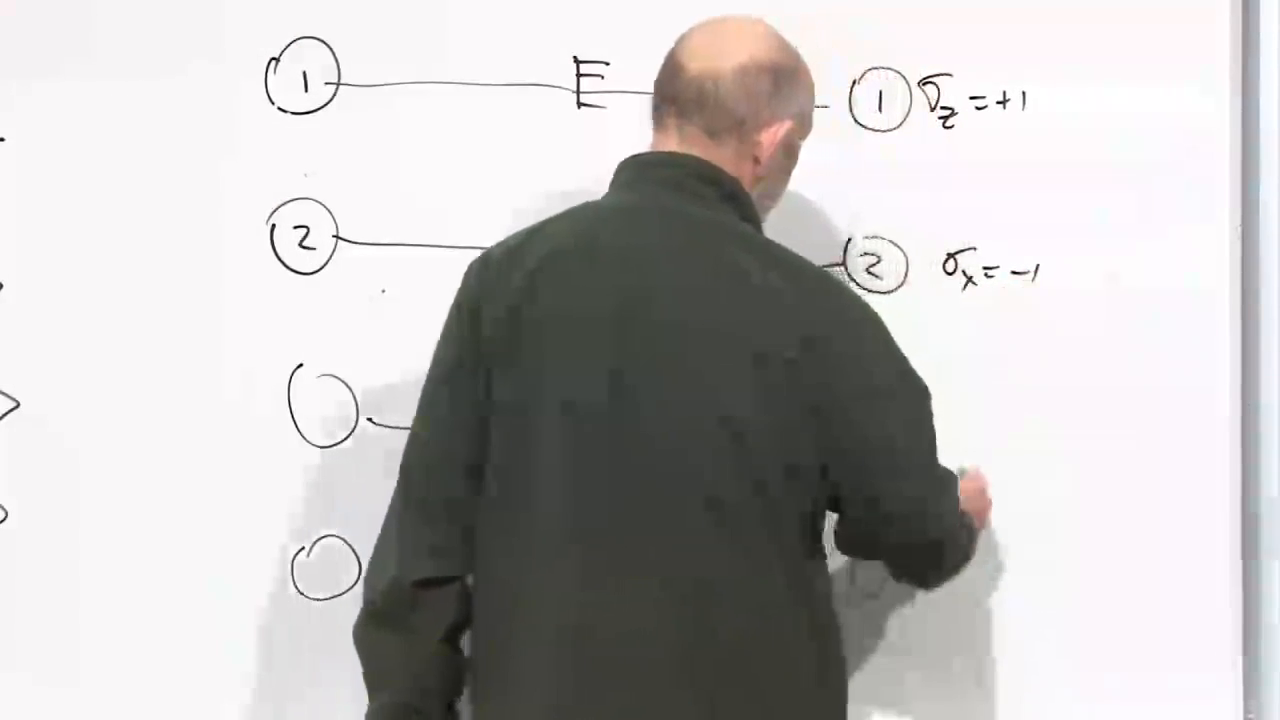
\includegraphics[width=0.88\textwidth]{lecture_07_figure_06.png}
\caption{Alice' Dichtematrix, erhalten durch Summation der gemeinsamen Amplituden über Bobs Basisbezeichnung.}
\lectureframe{01:02:33}
\end{figure}

Die reduzierte Dichtematrix ist hermitesch, positiv und normiert:
\begin{equation}
\rho_A^\dagger=\rho_A,
\qquad
\bra{\chi}\rho_A\ket{\chi}\geq0,
\qquad
\operatorname{Tr}\rho_A=1.
\label{eq:l7-density-properties}
\end{equation}
Sie enthält genau die Informationen, die für alle auf Alice beschränkten Messungen benötigt werden. Erzeugen zwei globale Zustände dasselbe \(\rho_A\), kann kein ausschließlich Alice betreffendes Experiment sie unterscheiden.

\begin{classroomqa}
\audiencequestion{Misst Alice die Dichtematrix als eine einzelne Observable?}
\lecturerresponse{Nicht in einer einzelnen Messung. Aus der Dichtematrix werden sämtliche Wahrscheinlichkeiten lokaler Messergebnisse berechnet. Bei vielen identisch präparierten Systemen kann Alice sie durch Tomografie rekonstruieren: Sie misst eine hinreichende Menge von Observablen und erschließt die Matrix aus deren Erwartungswerten.}
\end{classroomqa}

\begin{classroomqa}
\audiencequestion{Warum summiert man über Bob, statt einen von Bobs Zuständen auszuwählen?}
\lecturerresponse{Weil Alice keine Information über Bobs Messergebnis hat. Die partielle Spur summiert über eine vollständige Bob-Basis und liefert den unbedingten lokalen Zustand. Würde man stattdessen ein bestimmtes Messergebnis von Bob auswählen, erhielte man einen bedingten Zustand; das ist ein anderer Vorgang und setzt voraus, dass man dieses Ergebnis kennt.}
\end{classroomqa}

Für einen Produktzustand \(\Psi(a,b)=\psi_A(a)\phi_B(b)\) gilt
\begin{align}
(\rho_A)_{aa'}
&=\sum_b
\psi_A(a)\phi_B(b)
\psi_A^*(a')\phi_B^*(b) \\
&=\psi_A(a)\psi_A^*(a')
\sum_b|\phi_B(b)|^2 \\
&=\psi_A(a)\psi_A^*(a').
\end{align}
Damit ist
\begin{equation}
\rho_A=\ket{\psi_A}\bra{\psi_A}.
\label{eq:l7-pure-projector}
\end{equation}
Dies ist ein Projektor vom Rang eins. Auf \(\ket{\psi_A}\) angewandt, ergibt er
\begin{equation}
\rho_A\ket{\psi_A}
=\ket{\psi_A}\braket{\psi_A}{\psi_A}
=\ket{\psi_A},
\label{eq:l7-density-on-state}
\end{equation}
während er für jeden zu \(\ket{\psi_A}\) orthogonalen Zustand \(\ket{\chi}\) gilt
\begin{equation}
\rho_A\ket{\chi}
=\ket{\psi_A}\braket{\psi_A}{\chi}
=0.
\label{eq:l7-density-on-orthogonal}
\end{equation}

\begin{figure}[htbp]
\centering
\includegraphics[width=0.88\textwidth]{lecture_07_figure_07.png}
\caption{Eine Produktzustands-Dichtematrix wirkt als Projektor: Eigenwert \(1\) entlang \(\ket{\psi_A}\) und \(0\) für orthogonale Vektoren.}
\lectureframe{01:09:43}
\end{figure}

\section{Spektrum der Dichtematrix und Verschränkung}

Die Eigenwerte von \(\rho_A\) sind nichtnegativ und summieren sich zu eins. Für einen reinen Zustand des Gesamtsystems gilt:
\begin{itemize}
\item Genau ein von null verschiedener Eigenwert, gleich \(1\), bedeutet, dass der Zustand ein Produktzustand ist;
\item Mehr als ein von null verschiedener Eigenwert bedeutet, dass der Zustand verschränkt ist;
\item Gleiche Eigenwerte über den gesamten verfügbaren lokalen Träger bedeuten maximale Verschränkung.
\end{itemize}
Am klarsten zeigt sich dies anhand einer Schmidt-Zerlegung,
\begin{equation}
\begin{aligned}
\ket{\Psi}_{AB}
&=\sum_{r=1}^{R}\sqrt{\lambda_r}
\ket{r}_A\ket{r}_B,\\
\lambda_r&\geq0,
\qquad
\sum_r\lambda_r=1.
\end{aligned}
\label{eq:l7-schmidt}
\end{equation}
für die gilt
\begin{equation}
\rho_A=\sum_{r=1}^{R}\lambda_r\ket{r}_A\bra{r}.
\label{eq:l7-schmidt-density}
\end{equation}
Der Schmidt-Rang \(R\) beträgt bei einem Produktzustand eins und ist bei einem verschränkten reinen Zustand größer als eins.

Für den Singulettzustand gilt
\begin{equation}
\rho_A
=\operatorname{Tr}_B\ket{S}\bra{S}
=\frac12\ket{u}\bra{u}
+\frac12\ket{d}\bra{d}
=\frac12 I.
\label{eq:l7-singlet-reduced-density}
\end{equation}
Seine Eigenwerte sind
\begin{equation}
\operatorname{spec}(\rho_A)
=\left\{\frac12,\frac12\right\}.
\end{equation}
Alice' lokaler Zustand ist maximal gemischt, obwohl der Zustand des Paars rein ist.

Das Spektrum legt ein quantitatives Maß nahe. Die von-Neumann-Entropie
\begin{equation}
S(\rho_A)
=-\operatorname{Tr}(\rho_A\log\rho_A)
=-\sum_r\lambda_r\log\lambda_r
\label{eq:l7-entanglement-entropy}
\end{equation}verschwindet für einen reinen Produktzustand und erreicht bei einem maximal verschränkten Zustand \(\log d_A\), wenn \(d_A\leq d_B\). Auf die ausführliche Verwendung der Entropie können wir zunächst verzichten; schon das Spektrum liefert die wesentliche Unterscheidung.

\begin{classroomqa}
\audiencequestion{Muss jeder Eigenwert einer verschränkten reduzierten Dichtematrix von null verschieden sein?}
\lecturerresponse{Nein. Es genügt, dass mehr als ein Eigenwert von null verschieden ist. Ist Alice' Raum groß, kann ein verschränkter Zustand nur einen niedrigerdimensionalen Schmidt-Unterraum einnehmen, sodass weitere Eigenwerte null bleiben. Maximale Verschränkung bedeutet gleiche Eigenwerte über das gesamte kleinere Teilsystem hinweg, nicht bloß Gleichheit innerhalb einer beliebig ausgewählten Teilmenge.}
\end{classroomqa}

\begin{classroomqa}
\audiencequestion{Beweist eine gemischte reduzierte Dichtematrix für sich genommen, dass Alice mit Bob verschränkt ist?}
\lecturerresponse{Nur wenn bekannt ist, dass der globale Zustand rein ist. Ein gemischter lokaler Zustand kann auch aus einer gewöhnlichen klassischen Mischung in einem global gemischten Zustand hervorgehen. Bei einem reinen bipartiten Zustand ist lokale Mischung jedoch genau gleichbedeutend mit Verschränkung über die Bipartition hinweg.}
\end{classroomqa}

\begin{classroomqa}
\audiencequestion{Können alle Momente von Alice' Observablen ihre Wahrscheinlichkeitsverteilungen bestimmen?}
\lecturerresponse{In einem endlichdimensionalen System bestimmen die Erwartungswerte einer Operatorbasis \(\rho_A\), und \(\rho_A\) bestimmt über die Bornsche Regel jede lokale Ergebnisverteilung. Für die Rekonstruktion benötigt man ein Ensemble identisch präparierter Kopien; ein einzelnes isoliertes Ereignis kann keine Dichtematrix offenbaren.}
\end{classroomqa}

\section{Messung als verschränkende Wechselwirkung}

Ersetzen wir Alice und Bob durch einen Spin und eine Messapparatur. Die Apparatur habe einen Bereitschaftszustand \(\ket{0}_D\) und einen ausgelösten Zustand \(\ket{1}_D\). Eine ideale Wechselwirkung, die registriert, ob der Spin nach oben zeigt, lässt sich darstellen als
\begin{align}
\ket{u}\ket{0}_D&\longrightarrow\ket{u}\ket{1}_D,\\
\ket{d}\ket{0}_D&\longrightarrow\ket{d}\ket{0}_D.
\label{eq:l7-measurement-basis-map}
\end{align}
Der Detektor muss zunächst in einem bekannten Bereitschaftszustand sein; andernfalls wäre sein Endzustand kein eindeutiger Nachweis.

Die Linearität legt die Entwicklung einer Superposition fest:
\begin{equation}
\left(\alpha\ket{u}+\beta\ket{d}\right)\ket{0}_D
\longrightarrow
\alpha\ket{u}\ket{1}_D
+\beta\ket{d}\ket{0}_D.
\label{eq:l7-measurement-entanglement}
\end{equation}
Solange keiner der Koeffizienten verschwindet, ist der Endzustand verschränkt. Die Apparatur hat genau deshalb Information erhalten, weil ihr Zeigerzustand mit dem Spin korreliert ist.

\begin{figure}[htbp]
\centering
\includegraphics[width=0.88\textwidth]{lecture_07_figure_08.png}
\caption{Eine ideale Messung korreliert die Spin-Alternativen mit unterschiedlichen Zeigerzuständen und erzeugt dadurch Verschränkung.}
\lectureframe{01:20:20}
\end{figure}

Betrachtet man nur den Spin und ignoriert den Detektor, so lautet sein reduzierter Zustand
\begin{equation}
\rho_{\mathrm{spin}}
=|\alpha|^2\ket{u}\bra{u}
+|\beta|^2\ket{d}\bra{d},
\label{eq:l7-postmeasurement-reduced-state}
\end{equation}
sofern die Zeigeraufzeichnungen orthogonal sind. Die Interferenzterme sind aus der lokalen Beschreibung verschwunden, weil sie nun in den Korrelationen mit der Apparatur stecken.

Es gibt nun zwei einander ergänzende Beschreibungen. Wird das Detektorergebnis abgelesen und auf die Aufzeichnung konditioniert, ordnet man dem Spin den entsprechenden Zweig zu: \(\ket{u}\) nach einer Auslösung oder \(\ket{d}\), wenn keine Auslösung erfolgte. Das ist die Kollapsbeschreibung. Betrachtet man Detektor und Spin als ein geschlossenes System, ist Gleichung~\eqref{eq:l7-measurement-entanglement} eine gewöhnliche unitäre Entwicklung; aus dem gemeinsamen Zustand wurde kein Zweig entfernt.

\begin{classroomqa}
\audiencequestion{Ist Messung etwas, das über Verschränkung hinausgeht?}
\lecturerresponse{Auf der Ebene der System--Apparatur-Dynamik ist eine Messung eine Wechselwirkung, die eine verlässliche Korrelation herstellt. Der Kollaps ist die bedingte Beschreibung, die verwendet wird, nachdem eine bestimmte Aufzeichnung ausgewählt wurde. Ob man diese Aktualisierung als fundamental oder als relativ zu einer gewählten Schnittstelle auffasst, ist eine Interpretationsfrage; die operationalen Vorhersagen stimmen überein.}
\end{classroomqa}

\begin{classroomqa}
\audiencequestion{Warum lässt eine ideale Messung den Spin-Eigenzustand unverändert?}
\lecturerresponse{Das ist die Wiederholbarkeitsbedingung dieses Modells. Ist der Eingangszustand bereits ein Eigenzustand der gemessenen Observablen, soll die Apparatur ihren Wert registrieren, ohne ihn zu ändern. Reale Messungen können zerstörend sein; dann muss ihre Wechselwirkung jedoch anders modelliert werden.}
\end{classroomqa}

\section{Die Beobachterhierarchie}

Sobald die Apparatur als Quantensystem zugelassen ist, gibt es keinen natürlichen Grund, hier Halt zu machen. Licht vom Zeiger wechselwirkt mit einem Auge; Signale des Auges werden mit einem Gehirn korreliert; ein Beobachter kann von einem weiteren Beobachter beobachtet werden. Der Kater von Schr\"odinger und Wigners Freund veranschaulichen dieselbe verschachtelte Struktur:
\begin{equation}
\begin{gathered}
\text{spin}
\longrightarrow
\text{apparatus}
\longrightarrow
\text{cat}\\
\longrightarrow
\text{Schr\"odinger}
\longrightarrow
\text{Wigner}.
\end{gathered}
\label{eq:l7-observer-chain}
\end{equation}
Innerhalb jeder gewählten Grenze lässt sich die Kette durch unitäre Entwicklung und zunehmende Verschränkung beschreiben. Außerhalb der Grenze verwendet man die ergebnisbedingt formulierte Kollapsbeschreibung.

Die entscheidende Konsistenzbedingung lautet, dass sich die Grenze verschieben lässt. Registriert die Katze Spin nach oben, muss Schr\"odinger später eine Katze registrieren, die Spin nach oben gesehen hat, und Wigner muss Schr\"odinger dabei registrieren, dass dieser Verlauf aufgezeichnet wurde. Die Quantenmechanik legt keine eindeutige scharfe Linie fest, an der ein objektives Ereignis erklärt werden muss. Katzen, Augen und Gehirne bestehen aus physikalischen Freiheitsgraden; eines davon von der Quantenmechanik auszunehmen, würde ein zusätzliches Gesetz erfordern.

Feynman begegnete dem daraus entstehenden Unbehagen pragmatisch. Das begriffliche Problem kann so groß sein, dass schon schwer zu sagen ist, ob überhaupt eines vorliegt, während die Rechenregeln weiterhin jedes Experiment vorhersagen, auf das sie anwendbar sind. Der Formalismus soll keine bestimmte Interpretation erzwingen, sondern die Quelle des Unbehagens präzise herausarbeiten: Vollständige Kenntnis eines Ganzen kann damit einhergehen, dass es für seine Teile keine reine Zustandsbeschreibung gibt.

\begin{classroomqa}
\audiencequestion{Wenn ich die Katze bin, muss ich die Grenze dann bei mir selbst ziehen?}
\lecturerresponse{Für die eindeutige Aufzeichnung, die dir vorliegt, kannst du eine Kollapsbeschreibung verwenden. Ein anderer Beobachter, der dich in ein größeres isoliertes System einbezieht, kann eine Beschreibung durch einen verschränkten Zustand verwenden. Die Forderung ist nicht, dass alle dieselbe Grenze ziehen, sondern dass alle Beschreibungen übereinstimmende Aufzeichnungen liefern, wenn die Beobachter später ihre Ergebnisse vergleichen.}
\end{classroomqa}

\begin{classroomqa}
\audiencequestion{Wo tritt das objektive Ereignis ein: beim Atom, bei der Katze, bei Schr\"odinger oder bei Wigner?}
\lecturerresponse{Der unitäre Formalismus wählt keinen dieser Orte als privilegierte Grenze aus. Vielleicht werden gewöhnliche Wörter wie \emph{geschehen} über den Kontext hinaus verwendet, in dem sie präzise sind. Die formalen Werkzeuge sagen uns, wie sich Korrelationen ausbreiten und was jeder Beobachter vorhersagen kann; zu entscheiden, wie die endgültige Grenzziehung zu deuten ist, bleibt eine separate Aufgabe.}
\end{classroomqa}

\subsection{Schwache Kopplung und unvollkommene Auslesung}

Die ideale Zuordnung in Gleichung~\eqref{eq:l7-measurement-basis-map} erzeugt perfekt unterscheidbare Aufzeichnungen. Bei einer schwächeren Wechselwirkung sind die Apparaturzustände möglicherweise nur teilweise unterscheidbar:
\begin{equation}
\alpha\ket{u}\ket{D_u}
+\beta\ket{d}\ket{D_d},
\qquad
0<|\braket{D_d}{D_u}|<1.
\label{eq:l7-weak-measurement}
\end{equation}
Dann erhält die Apparatur nur teilweise Information, und die Verschränkung ist unvollständig. Dies ist der Fall einer schwachen oder unscharfen Messung.

Diese Situation muss von einer mangelhaften nachgelagerten Auslesung unterschieden werden. Der Detektor kann bereits vollständig mit dem Spin korreliert sein, während Auge, Kabel, Verstärker oder Gehirn die Aufzeichnung nicht zuverlässig übermitteln. Im ersten Fall ist die Wechselwirkung zwischen System--Detektor schwach; im zweiten liegt beim Detektor eine gute Aufzeichnung vor, aber die spätere Informationsübertragung ist ineffizient. Die Detektoreffizienz kann beide Stufen betreffen; deshalb muss man zuerst die physikalische Kopplung bestimmen, bevor man die Ursache zuordnet.

\begin{classroomqa}
\audiencequestion{Wenn das Sehvermögen eingeschränkt ist und sich der Zeigerstand deshalb nicht sicher ablesen lässt: War die quantenmechanische Messung dann schwach?}
\lecturerresponse{Nicht unbedingt. Der Spin kann stark und vollständig mit dem Messgerät korreliert gewesen sein, während die Übertragung vom Gerät zum Auge oder vom Auge zum Gehirn gestört war. Bei einer tatsächlich schwachen Messung erzeugt bereits die anfängliche Kopplung zwischen System--Apparat nur teilweise unterscheidbare Anzeigen.}
\end{classroomqa}

\section{Lokalität und Signalübertragung}

Der Ausdruck \emph{Fernwirkung} sollte operational definiert werden. In der gewöhnlichen Physik verändert eine Einwirkung aus der Ferne, was hier beobachtet werden kann. Würde die Sonne verschwinden und sich die Bewegung der Erde sofort ändern, statt erst nach der Lichtlaufzeit, ließe sich diese Änderung nutzen, um Information schneller als Licht zu übertragen. Das wäre echte nichtlokale Signalübertragung.

Verschränkung ermöglicht keine solche Signalübertragung. Bob führe eine lokale Quantenoperation aus, die durch Kraus-Operatoren \(K_\mu\) dargestellt wird, mit
\begin{equation}
\sum_\mu K_\mu^\dagger K_\mu=I_B.
\end{equation}
Wenn Alice nicht erfährt, welches Ergebnis Bob erhält, lautet der endgültige gemeinsame Zustand
\begin{equation}
\rho'_{AB}
=\sum_\mu
(I_A\otimes K_\mu)\rho_{AB}
(I_A\otimes K_\mu^\dagger).
\end{equation}
Die partielle Spur über Bob ergibt
\begin{equation}
\rho'_A
=\operatorname{Tr}_B\rho'_{AB}
=\operatorname{Tr}_B\rho_{AB}
=\rho_A.
\label{eq:l7-no-signaling}
\end{equation}
Damit bleibt jede unbedingte lokale Wahrscheinlichkeit für Alice unverändert, wenn Bob eine spurtreue lokale Operation wählt.

Bedingte Zustände sind etwas anderes. Wenn Bob misst und das Ergebnis \(\mu\) erhält, kann Alice den Zustand
\begin{equation}
\rho_{A|\mu}
=\frac{
\operatorname{Tr}_B\!\left[
(I_A\otimes K_\mu)\rho_{AB}
(I_A\otimes K_\mu^\dagger)
\right]
}{p_\mu}.
\label{eq:l7-conditioned-state}
\end{equation}
zuordnen. Doch Alice kann nicht wissen, welcher Zustand \(\rho_{A|\mu}\) gilt, bis Bob ihr \(\mu\) durch ein gewöhnliches Signal mitteilt. Bevor die Nachricht eintrifft, muss sie über die Ergebnisse mitteln:
\begin{equation}
\sum_\mu p_\mu\rho_{A|\mu}=\rho_A.
\label{eq:l7-conditioned-average}
\end{equation}

\begin{classroomqa}
\audiencequestion{Wann ändert sich Alices Dichtematrix, wenn Bob zuerst misst?}
\lecturerresponse{Ihre unbedingte Dichtematrix ändert sich nicht. Sobald Bobs Ergebnis sie erreicht, kann sie sie durch die entsprechende bedingte Dichtematrix ersetzen. Diese Aktualisierung spiegelt neu verfügbare Information wider und kann nicht erfolgen, bevor die klassische Nachricht eintrifft.}
\end{classroomqa}

\begin{classroomqa}
\audiencequestion{Lässt Bobs Messung Alices Zustand physikalisch im selben Augenblick kollabieren?}
\lecturerresponse{Die verschiedenen Interpretationen beschreiben die bedingte Aktualisierung unterschiedlich, doch sie stimmen alle in der überprüfbaren Aussage überein: Alices lokale Ergebniswahrscheinlichkeiten bleiben unverändert, bis ihr Information von Bob vorliegt. Es entsteht kein kontrollierbares instantanes Signal.}
\end{classroomqa}

Stellen wir uns viele Singulettpaare vor, die auf nummerierte Zeilen verteilt sind. Bei einem Partner misst Bob \(z\), bei einem anderen \(x\), bei einem weiteren \(y\) und so weiter. Alices lokale Ergebnisse bleiben in jeder Zeile eine unverzerrte Folge:
\begin{equation}
P_A(+|\mathbf a)=P_A(-|\mathbf a)=\frac12.
\label{eq:l7-alice-marginal}
\end{equation}
Nichts in ihrem Notizbuch verrät, welche Achsen Bob gewählt oder welche Ergebnisse er erhalten hat.

\begin{figure}[htbp]
\centering
\includegraphics[width=0.88\textwidth]{lecture_07_figure_09.png}
\caption{Viele unabhängig präparierte Paare ermöglichen es, verschiedenen Zeilen unterschiedliche Messachsen zuzuweisen; Alices Randstatistik bleibt unverändert.}
\lectureframe{01:49:00}
\end{figure}

Nachdem ein auf Lichtgeschwindigkeit begrenztes Telegramm eingetroffen ist, das Bobs Achse und Ergebnis für jede Zeile auflistet, kann Alice ihre Aufzeichnungen sortieren. Bei Messungen entlang derselben Achse sind die Ergebnisse der Singulettpartner dann für jedes Paar entgegengesetzt. Die Nachricht macht Korrelationen sichtbar, die bereits in der gemeinsamen Statistik enthalten waren; sie verändert Alices frühere lokale Häufigkeitsverteilung nicht rückwirkend.

\begin{classroomqa}
\audiencequestion{Könnte Alice Bobs Wahl aus genügend vielen Momenten ihrer eigenen Daten erschließen?}
\lecturerresponse{Alle lokalen Momente von Alice sind durch \(\rho_A\) festgelegt, und Gleichung~\eqref{eq:l7-no-signaling} lässt diese Matrix unverändert. Mehr Kopien verbessern ihre Schätzung derselben lokalen Dichtematrix; sie verraten weder Bobs Basis noch sein Ergebnis.}
\end{classroomqa}

\begin{classroomqa}
\audiencequestion{Was geschieht, wenn Bob für jedes Ensemblemitglied eine andere Achse wählt?}
\lecturerresponse{Alice beobachtet weiterhin dieselbe lokale Verteilung. Sobald Bob ihr die Einstellungen und Ergebnisse für jede Zeile mitteilt, können beide die bedingten Korrelationen für jedes Achsenpaar vergleichen. Die Abhängigkeit von den Einstellungen zeigt sich in der gemeinsamen Statistik, nicht in Alices Randstatistik.}
\end{classroomqa}

\section{Bells Frage als Simulationsspiel}

Der Unterschied zwischen dem Ausbleiben von Signalübertragung und Bell-Nichtlokalität wird als Problem der klassischen Simulation klarer. Betrachten wir zunächst einen Spin,
\begin{equation}
\ket{\psi}=\alpha_u\ket{u}+\alpha_d\ket{d},
\qquad
|\alpha_u|^2+|\alpha_d|^2=1.
\end{equation}
Ein klassisches Programm kann die beiden komplexen Amplituden speichern, sie mit der Schr\"odinger-Gleichung entwickeln und eine vom Nutzer gewählte Messrichtung entgegennehmen. Wird der Messbefehl ausgeführt, berechnet das Programm die Born-Wahrscheinlichkeiten, wählt mithilfe eines Pseudozufallszahlengenerators ein Ergebnis aus, zeigt es an und aktualisiert den gespeicherten Zustand auf den entsprechenden Eigenzustand. Bei wiederholter Ausführung reproduziert es die Statistik eines einzelnen Spins.

Zufälligkeit allein ist also nicht das Unterscheidungsmerkmal zwischen klassischer und Quantenmechanik. Klassische Computer können Folgen erzeugen, die für eine Simulation operational hinreichend zufällig sind, selbst wenn ihre Pseudozufallsalgorithmen im Hintergrund deterministisch sind.

Für zwei Spins in einem Produktzustand genügen ebenfalls zwei getrennte Computer. Alices Computer speichert und entwickelt \(\ket{\psi_A}\); Bobs speichert und entwickelt \(\ket{\phi_B}\). Jeder reagiert nur auf seine lokale Einstellung. Da die gemeinsamen Wahrscheinlichkeiten faktorisieren, ist nach der Trennung der Computer keine Kommunikation erforderlich.

Ein verschränktes Paar verändert das Problem. Man kann die beiden Maschinen vor dem Experiment zusammenbringen, korrelierte verborgene Daten laden, ihre Uhren synchronisieren und ihnen sogar identische Zufallszahlenfolgen vorgeben. Nach ihrer Trennung muss jedes Ergebnis jedoch ausschließlich von der lokalen Messeinstellung und den im Voraus bereitgestellten gemeinsamen Informationen abhängen. Bells Theorem zeigt, dass kein solches lokales Modell mit verborgenen Variablen alle Quantenkorrelationen für frei gewählte Einstellungen reproduzieren kann.

\begin{figure}[htbp]
\centering
\includegraphics[width=0.88\textwidth]{lecture_07_figure_10.png}
\caption{Das Modell getrennter Computer: Die lokalen Programme können Präparationsdaten gemeinsam nutzen, nach der Trennung aber nicht über Messeinstellungen kommunizieren.}
\lectureframe{02:00:00}
\end{figure}

Bleiben Leitungen zwischen den Computern bestehen, über die Einstellungen und Ergebnisse ausgetauscht werden können, lässt sich die Simulation so einrichten, dass sie die Korrelationen reproduziert. Dann bilden die beiden Computer jedoch kein wirklich getrenntes lokales Modell mehr, sondern funktionieren als ein verbundener Computer. Das Hindernis liegt nicht in der klassischen Berechnung an sich. Eine einzelne globale klassische Maschine kann endliche Quantensysteme simulieren, indem sie die vollständige gemeinsame Wellenfunktion speichert, auch wenn der erforderliche Speicher im Allgemeinen exponentiell mit der Zahl der Teilsysteme wächst. Bells Hindernis betrifft die Zerlegung in unabhängig arbeitende lokale Maschinen.

\begin{classroomqa}
\audiencequestion{Warum können die beiden Computer nicht einfach dieselbe Folge von Zufallszahlen verwenden?}
\lecturerresponse{Gemeinsam genutzte Zufälligkeit ist in einem lokalen Modell mit verborgenen Variablen bereits zugelassen. Sie kann korrelierte Antworten vorab festlegen, doch jede Antwort muss für alle Messeinstellungen funktionieren, die später auf der jeweiligen Seite gewählt werden könnten. Bell-Ungleichungen geben die Bedingungen an, denen alle derartigen vorab festgelegten lokalen Strategien genügen; die Quantenkorrelationen verletzen diese Bedingungen.}
\end{classroomqa}

\begin{classroomqa}
\audiencequestion{Müssen die Zufallszahlen von den Messrichtungen abhängen?}
\lecturerresponse{Ein lokales Ergebnis darf von der eigenen lokalen Richtung und den gemeinsam genutzten verborgenen Daten abhängen, nicht aber von der entfernten Richtung, die nach der Trennung gewählt wird. Eine Abhängigkeit von beiden Einstellungen setzt Kommunikation, Rückwärtskausalität oder eine Verletzung der üblichen Annahme der Messunabhängigkeit voraus. Bells Theorem macht diese Annahmen explizit, statt sie im Wort \emph{zufällig} zu verbergen.}
\end{classroomqa}

\begin{classroomqa}
\audiencequestion{Wären zwei getrennte Quantencomputer erfolgreich, wo die klassischen Programme scheitern?}
\lecturerresponse{Sie können erfolgreich sein, wenn sie verschränkte quantenmechanische Freiheitsgrade gemeinsam nutzen. In diesem Fall simulieren die Computer Verschränkung nicht mithilfe lokaler klassischer Aufzeichnungen, sondern besitzen sie physikalisch. Ihre lokalen Ergebnisse können weiterhin keine kontrollierbare Nachricht schneller als Licht übertragen.}
\end{classroomqa}

\begin{classroomqa}
\audiencequestion{Kann ein gewöhnlicher klassischer Computer das gesamte Paar simulieren?}
\lecturerresponse{Ja. Er kann die vier gemeinsamen Amplituden speichern und alle Messwahrscheinlichkeiten an einem Ort berechnen. Bei vielen Teilchen wird diese direkte Simulation aufwendig, weil die Dimension des Hilbertraums exponentiell wächst; ein Widerspruch zu Bell entsteht jedoch nicht, wenn alle Informationen innerhalb einer einzigen Maschine global verfügbar sind.}
\end{classroomqa}

\begin{classroomqa}
\audiencequestion{Beweist Bells Theorem also eine gewöhnliche Fernwirkung?}
\lecturerresponse{Es beweist, dass lokale Erklärungen mit verborgenen Variablen, die Bells Annahmen erfüllen, die beobachteten Korrelationen nicht reproduzieren können. Es stellt Alice oder Bob keinen überlichtschnellen Signalweg zur Verfügung. Bell-Nichtlokalität und operationale Kommunikation schneller als Licht sind zwei verschiedene Aussagen.}
\end{classroomqa}

\section{Was sich lokal erfahren lässt}

Lokale und gemeinsame Observablen dürfen nicht miteinander verwechselt werden. Bob kann \(\sigma_x\) messen und Alice \(\tau_x\); durch den späteren Vergleich ihrer Aufzeichnungen schätzen sie
\begin{equation}
\expect{\sigma_x\tau_x}.
\end{equation}
Keine der beiden lokalen Apparaturen misst für sich allein dieses Produkt. Der rotationsskalare Ausdruck
\begin{equation}
\boldsymbol{\sigma}\cdot\boldsymbol{\tau}
=\sigma_x\tau_x+\sigma_y\tau_y+\sigma_z\tau_z
\end{equation}
erfordert entweder verschiedene Teilensembles für die drei Terme oder eine neue gemeinsame Apparatur, die die Singulett- und Triplettsektoren auflöst. Mit den ursprünglichen lokalen Spinmessgeräten lassen sich nicht alle drei inkompatiblen Komponentenprodukte an einem einzelnen Paar bestimmen.

\begin{classroomqa}
\audiencequestion{Gibt es Observablen des Gesamtsystems, die Alice und Bob mit ihren ursprünglichen Apparaturen nicht getrennt messen können?}
\lecturerresponse{Ja. Ein einzelnes Produkt wie \(\sigma_x\tau_x\) lässt sich durch zwei lokale Messungen von \(x\) schätzen, gefolgt von einem Vergleich. Die Summe \(\boldsymbol{\sigma}\cdot\boldsymbol{\tau}\) lässt sich nicht aus gleichzeitig vorgenommenen Messungen von \(x,y,z\) an einem einzelnen Paar zusammensetzen. Dafür braucht man eine echte gemeinsame Messung der Singulett--Triplettsektoren oder getrennte Ensembles für die inkompatiblen Terme.}
\end{classroomqa}

Bob kann Verschränkung nicht aus einem einzelnen Ereignis ableiten. An vielen identisch präparierten Kopien kann er jedoch seine reduzierte Dichtematrix rekonstruieren. Für ein Qubit gilt
\begin{equation}
\rho_B
=\frac12\left(
I+\mathbf r\cdot\boldsymbol{\sigma}
\right),
\label{eq:l7-bloch-density}
\end{equation}
und Messungen entlang mehrerer Achsen bestimmen den Bloch-Vektor \(\mathbf r\). Wenn \(|\mathbf r|=1\), ist Bobs lokaler Zustand rein; wenn \(|\mathbf r|<1\), ist er gemischt. Im besonderen Fall, dass bekannt ist, dass die globale Präparation in jedem Versuch derselbe reine Zustand ist, beweist die lokale Gemischtheit, dass Bob mit etwas außerhalb seines Teilsystems verschränkt ist.

Bei einem Produkt zweier reiner Spins kann Bob nach der Polarisationsrichtung \(\mathbf n=\mathbf r/|\mathbf r|\) suchen. Bei wiederholten Messungen entlang dieser Achse erhält er stets ein eindeutiges Ergebnis. Für das Singulett gilt \(\mathbf r=0\), sodass jede Achse lokal zufällige Ergebnisse liefert. Bei der Suche findet sich keine Polarisationsrichtung.

\begin{classroomqa}
\audiencequestion{Kann Bob Verschränkung entdecken, ohne mit Alice zu sprechen?}
\lecturerresponse{Anhand eines Ensembles kann er feststellen, dass sein eigener reduzierter Zustand gemischt ist. Weiß er außerdem, dass jedes Paar im selben globalen reinen Zustand präpariert wurde, kann er auf Verschränkung über die Grenze seines Teilsystems hinweg schließen. Ohne diese Reinheitsannahme könnte sein gemischter Zustand stattdessen auf eine klassische Präparationsmischung zurückgehen; dann ließe sich die Unterscheidung allein anhand lokaler Daten nicht klären.}
\end{classroomqa}

\begin{classroomqa}
\audiencequestion{Warum braucht man viele identisch präparierte Systeme?}
\lecturerresponse{Jede Spinmessung liefert nur ein Ergebnis und stört im Allgemeinen die jeweilige Kopie. Für die Tomografie verteilt man inkompatible Messungen daher auf ein Ensemble, das nach demselben Verfahren präpariert wurde. Die Dichtematrix und ihr Spektrum sind statistische Eigenschaften, die aus wiederholten Versuchen erschlossen werden, und keine Merkmale, die ein einzelnes Teilchen offenbart.}
\end{classroomqa}

Damit schließt sich der Gedankengang an seinen Ausgangspunkt an. Verschränkung ist kein vages Teilen eines Zustands. Sie liegt vor, wenn ein reiner gemeinsamer Zustand nicht faktorisiert; lokal zeigt sich das in einer reduzierten Dichtematrix, die kein Projektor ist, und gemeinsam in Korrelationen, die sich nicht durch getrennte klassische Buchführung reproduzieren lassen. Das Ganze kann vollständig bekannt sein, während jeder Teil gemischt bleibt. Dadurch wird Messung möglich, die Signalübertragung bleibt ausgeschlossen, und es entsteht die Struktur, die Bells Theorem prüfen wird.
